\documentclass[11pt]{article}
\usepackage[utf8]{inputenc}
\usepackage[english]{babel}
\usepackage{bilal2vec}

\title{CS 370 - A1}
\author{Bilal Khan\\
\href{mailto:bilal2vec@gmail.com}{bilal2vec@gmail.com}}
\date{\today}

\begin{document}

\maketitle

\tableofcontents

\section{1}

\subsection{a}

The smallest value is given by $(0.10000)_{4} \times 4^{-10}$. The largest value is given by $(0.33333)_{4} \times 4^{10}$.

\subsection{b}

$(0.0321223)_4 / (10)_4 = (0.0321223)_4 \times 4^{-1} = (0.321223)_4 \times 4^{-2}$. The mantissa here has 6 digits and has to be rounded to 5 digits. Since the 6th digit (3) is larger than half the maximum significand (2), we round up. The result is $(0.32123)_4 \times 4^{-2}$.

\subsection{c}

Machine epsilon is given by $\dfrac{1}{2} \beta^{-(m - 1)}$. In this case, $\beta = 4$ and $m = 5$ and machine epsilon is given by $\dfrac{1}{2} \times 4^{-4}$.

\subsection{d}

All values in this number system where the exponent $p \leq 0$ are smaller than one. There are 21 possible exponents in $[-10, 10]$ and so $11/21$ of the numbers are smaller than one.

\section{2}

Given a machine epsilon E, $f(\bar{x} \ominus \bar{y}) = (\bar{x} - \bar{y})(1 + E)$, and $f(\bar{x} \otimes \bar{y}) = (\bar{x} \times \bar{y})(1 + E)$, We can find the relative error of the whole expression.

\[ f(y \ominus 1) = (y - 1) (1 + E) \]
\[ f(y \oplus 1) = (y + 1) (1 + E) \]
\[ f(x \otimes y) = (x \times y) (1 + E) \]

\begin{align*}
    f((y \ominus 1) \otimes (y \oplus 1)) &= (((y - 1) (1 + E)) \times ((y + 1) (1 + E)))(1 + E) \\
    &= ((y-1)(1+E)(y+1)(1+E))(1 + E) \\
    &= ((y-1)(y+1)(1+E)(1+E))(1 + E) \\
    &= ((y^2 - y + y - 1)(1^2 + 2E + E^2))(1 + E) \\
    &= (y^2 - 1)(1 + 2E + E^2)(1 + E) \\
    &= (y^2 - 1)(1 + 2E + E^2 + E + 2E^2 + E^3) \\
    &= (y^2 - 1)(1 + 3E + 3E^2 + E^3) \\
\end{align*}

The bound on the relative error is then $3E + 3E^2 + E^3$.

\section{3}

\subsection{a}

\begin{minted}{python}
import math

def PowerSin(x):
  idx = 1
  exp = 3
  sum = 0
  term = x

  while sum + term != sum:
    sum = sum + term
    term = ((-1)**idx) * (x**exp) / math.factorial(exp)

    idx += 1
    exp += 2
  
  return sum
\end{minted}

\subsection{b}

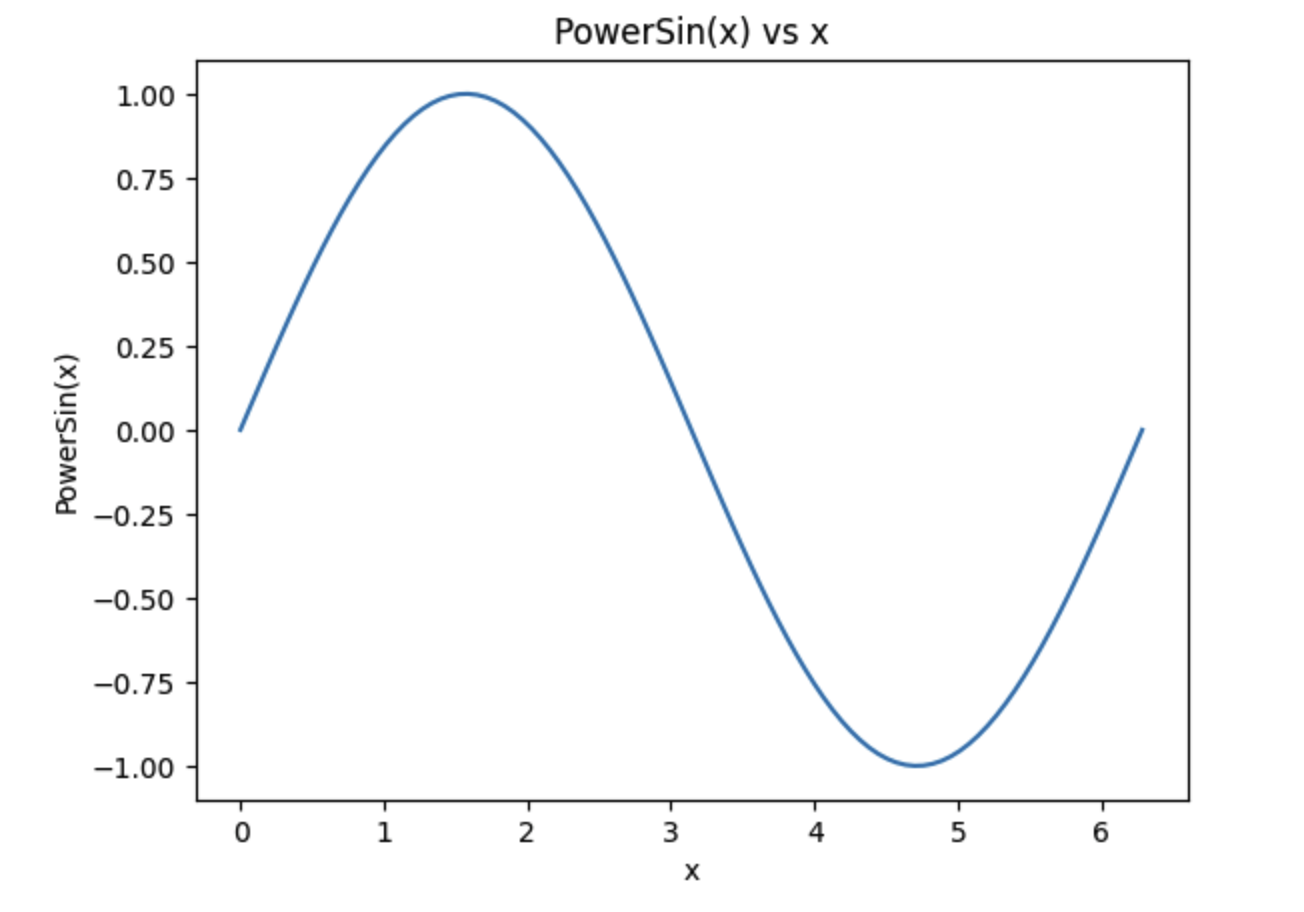
\includegraphics[width=300pt]{a1-3b.png}

\subsection{c}

\begin{table}[h]
    \centering
    \begin{tabular}{|c|c|c|c|c|}
    \hline
    \( x \) & \text{PowerSin(x)} & \text{sin(x)} & \text{Error} & \text{Number of Terms} \\
    \hline
    $ \pi /2 $    & $1.0000000000000002$ & $1.0$  & $0.0000000000000002$ & 11 \\
    $ 11\pi / 2 $ & $-1.000000000155901$ & $-1.0$ & $0.000000000155901$  & 37 \\
    $ 21\pi / 2 $ & $1.0046249045393962$ & $1.0$  & $0.0046249045393962$ & 59 \\
    $ 31\pi / 2 $ & $17863.02585515233$  & $-1.0$ & $17864.02585515233$  & 77 \\
    \hline
    \end{tabular}
\end{table}

\subsection{d}

At sufficiently large values, the floating point errors become large enough that the power series no longer converges to the correct value. This can be fixed in a way for this example by always computing \mintinline{python}{PowerSin(x % (2 * math.pi))} since the sin function is periodic.

\section{4}

\section{5}

\section{6}

\section{7}

\end{document}
